% This file was created by tikzplotlib v0.9.8.
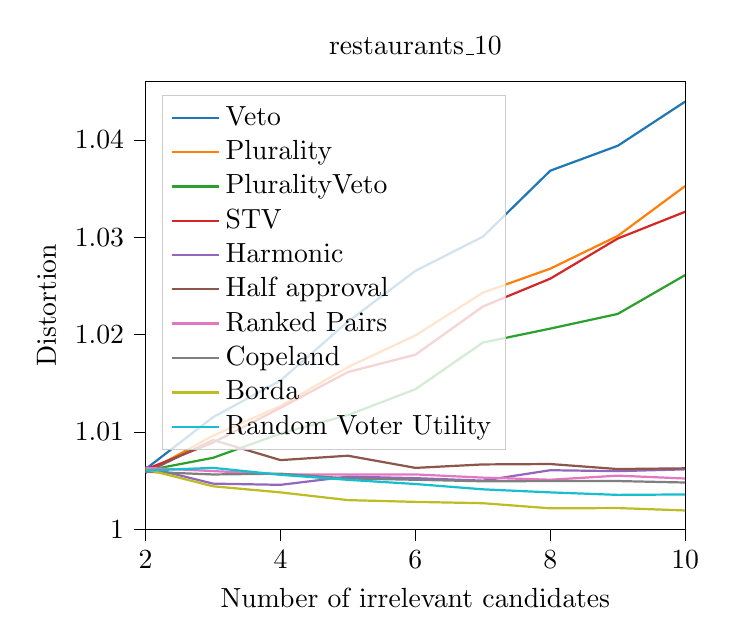
\begin{tikzpicture}

\definecolor{color0}{rgb}{0.12156862745098,0.466666666666667,0.705882352941177}
\definecolor{color1}{rgb}{1,0.498039215686275,0.0549019607843137}
\definecolor{color2}{rgb}{0.172549019607843,0.627450980392157,0.172549019607843}
\definecolor{color3}{rgb}{0.83921568627451,0.152941176470588,0.156862745098039}
\definecolor{color4}{rgb}{0.580392156862745,0.403921568627451,0.741176470588235}
\definecolor{color5}{rgb}{0.549019607843137,0.337254901960784,0.294117647058824}
\definecolor{color6}{rgb}{0.890196078431372,0.466666666666667,0.76078431372549}
\definecolor{color7}{rgb}{0.737254901960784,0.741176470588235,0.133333333333333}
\definecolor{color8}{rgb}{0.0901960784313725,0.745098039215686,0.811764705882353}

\begin{axis}[
legend cell align={left},
legend style={
  fill opacity=0.8,
  draw opacity=1,
  text opacity=1,
  at={(0.03,0.97)},
  anchor=north west,
  draw=white!80!black
},
tick align=outside,
tick pos=left,
title={restaurants\_10},
x grid style={white!69.0196078431373!black},
xlabel={Number of irrelevant candidates},
xmin=2, xmax=10,
xtick style={color=black},
y grid style={white!69.0196078431373!black},
ylabel={Distortion},
ymin=1, ymax=1.04605044808658,
ytick style={color=black}
]
\addplot [thick, color0]
table {%
2 1.00619681961188
3 1.01153054179347
4 1.01529216818569
5 1.02135250218871
6 1.02656038233964
7 1.03006879736373
8 1.03685095538422
9 1.03940819492308
10 1.04395034577876
};
\addlegendentry{Veto}
\addplot [thick, color1]
table {%
2 1.00583370284813
3 1.00962659584734
4 1.01267215099024
5 1.01667477513015
6 1.01992807249546
7 1.02431901312952
8 1.02678599418981
9 1.03015106571984
10 1.03527752739326
};
\addlegendentry{Plurality}
\addplot [thick, color2]
table {%
2 1.0060338431186
3 1.00735542564608
4 1.00984472583763
5 1.01174553415003
6 1.01440229527779
7 1.01919230331087
8 1.02062771374408
9 1.02213752694973
10 1.02613077286696
};
\addlegendentry{PluralityVeto}
\addplot [thick, color3]
table {%
2 1.00615773405231
3 1.0089213856489
4 1.01248559278942
5 1.0161687096721
6 1.01794984024418
7 1.02289689361547
8 1.02576087813236
9 1.02988297251692
10 1.03263262328025
};
\addlegendentry{STV}
\addplot [thick, color4]
table {%
2 1.00641707170896
3 1.00470460958613
4 1.00458085768813
5 1.00542396267518
6 1.00526714465335
7 1.00501076604302
8 1.0060820458062
9 1.00598743559916
10 1.00617077804312
};
\addlegendentry{Harmonic}
\addplot [thick, color5]
table {%
2 1.00583905038105
3 1.00918665245463
4 1.0071200880568
5 1.00757172449762
6 1.00632257448155
7 1.00667683906483
8 1.00671875199406
9 1.00620274653223
10 1.00627757258442
};
\addlegendentry{Half approval}
\addplot [thick, color6]
table {%
2 1.00632720751813
3 1.00599367448993
4 1.00565816477584
5 1.0056449024503
6 1.00564915467401
7 1.00532190858346
8 1.00510530223207
9 1.00552560839376
10 1.00522999714347
};
\addlegendentry{Ranked Pairs}
\addplot [thick, white!49.8039215686275!black]
table {%
2 1.00592384925919
3 1.00564692192655
4 1.00572493704135
5 1.00523813550443
6 1.00510011000471
7 1.00494585287663
8 1.0049686835025
9 1.00497005773595
10 1.00481995114301
};
\addlegendentry{Copeland}
\addplot [thick, color7]
table {%
2 1.00618387460312
3 1.00443223514934
4 1.0038077659107
5 1.0030115321341
6 1.00283049005392
7 1.00269428924145
8 1.00216961665512
9 1.00219591108807
10 1.00194829962235
};
\addlegendentry{Borda}
\addplot [thick, color8]
table {%
2 1.00604498574929
3 1.00632528175455
4 1.00561238838424
5 1.00509442140486
6 1.00466588838139
7 1.00411969522506
8 1.00380599324025
9 1.0035494650803
10 1.00359260882355
};
\addlegendentry{Random Voter Utility}
\end{axis}

\end{tikzpicture}
